\chapter{Rappels théoriques sur les interfaces}
{\color{red} mettre le bruit systémaiquement à chaque équation, rappeler le bruit}
{\color{red} être sûr de définir tous les nouveaux mots. Revoir 1.64, cisaillement, quj'est-ce que v ?}
{\color{red} séparer ce qu'on fait les autres et ce que j'ai fait moi-même.}
{\color{red} faire gaffe quand ce sont des vecteurs et non des scalaires !!!}
 {\color{red} changer les exponentielles en exponentielles complètes. Ajouter de l'effet Casimir critique de Cardozo avec discussion thermodynamique.}
  
Dans ce chapitre nous analysons la dynamique des systèmes statistiques. L'analyse nous permettra de comprendre comment les transitions de phase, notament certains systèmes subissant une séparation de phase à la transition, se comportent de manière dynamique. L'exemple le plus connu est le modèle d'Ising en absence de champ magnétique, ayant la magnétisation comme paramètre d'ordre de la transition. Dans la phase haute température le système est homogène et sa magnétisation est nulle, tandis qu'en dessous de la température critique, dans le cas où le paramètre d'ordre est conservé (par exemple une dynamique de Kawasaki ou modèle B), le système va localement se séparer en deux phases de magnétisation moyenne opposée séparées par une interface minimisant l'énergie de surface entre les deux phases. 
Dans le cas où le paramètre d'ordre n'est pas conservé (par exemple une dynamique de Glauber ou modèle A), une brisure spontannée de symmétrie fera que l'une des deux phases englobe l'autre, au point de recouvrir tout le système (voir Fig \ref{clusterization}). Dans une transition de phase continue où le point critique est atteint depuis l'état désordonné vers l'état ordonné, les domaines de phase égales ont pour taille la longueur de corrélation du système. Dans les transitions de phase telles que celles du modèle d'Ising, la longueur de corrélation diverge lorsque l'on s'approche de la température critique $T_C$. En présence d'un système infini, la longueur de corrélation devient infinie, ce qui implique que le système prend un temps infini pour atteindre l'équilibre thermodynamique. Ce processus de croissance des domaines depuis la phase désordonnée s'appelle le \textit{coarsening} et la théorie de la cinétique d'ordre des phases est la théorie qui a été développée pour le comprendre.
Cette thèse s'appuie cette théorie pour déterminer les propriétés statistiques (telles que la position moyenne et sa tension superficielle) des interfaces entre deux phases coexistantes.

Tandis que l'Hamiltonien d'un système permet d'explorer toutes les configurations d'équilibre possibles, la dynamique du coarsening ne peut être étudiée qu'en construisant un modèle qui explique l'évolution de l'état du système en fonction du temps. Nous verrons tout au long de ce travail comment la conservation (ou non) du paramètre d'ordre influe sur la dynamique. Nous nous référons principalement dans ce chapitre aux références \cite{hohenberg_theory_1977,bray_theory_1994,krapivsky_kinetic_2010,halpin-healy_kinetic_1995}.

Une connaissance parfaite de la fonction de partition nécessite de connaître toutes les micro-configurations possibles du système. Les appareils de mesure possèdent tous une résolution spatiale et temporelle, c'est-à-dire qu'ils mesurent l'état moyen de toutes les particules dans un volume et dans un laps de temps donné. Plus la résolution des appareils de mesure est bonne, et plus la mesure des observables dérivées de la fonction de partition est précise. 
Concrètement, l'appareil de mesure nous donne un champ - par exemple de densité - $\phi(\mx,t)$ de notre système, qui correspond à l'intégration sur un petit volume autour de $\mx$ et une petite durée de temps autour de $t$.
{\color{red} mettre équation coarse-graining} 

\begin{figure}[h]
    \centering
    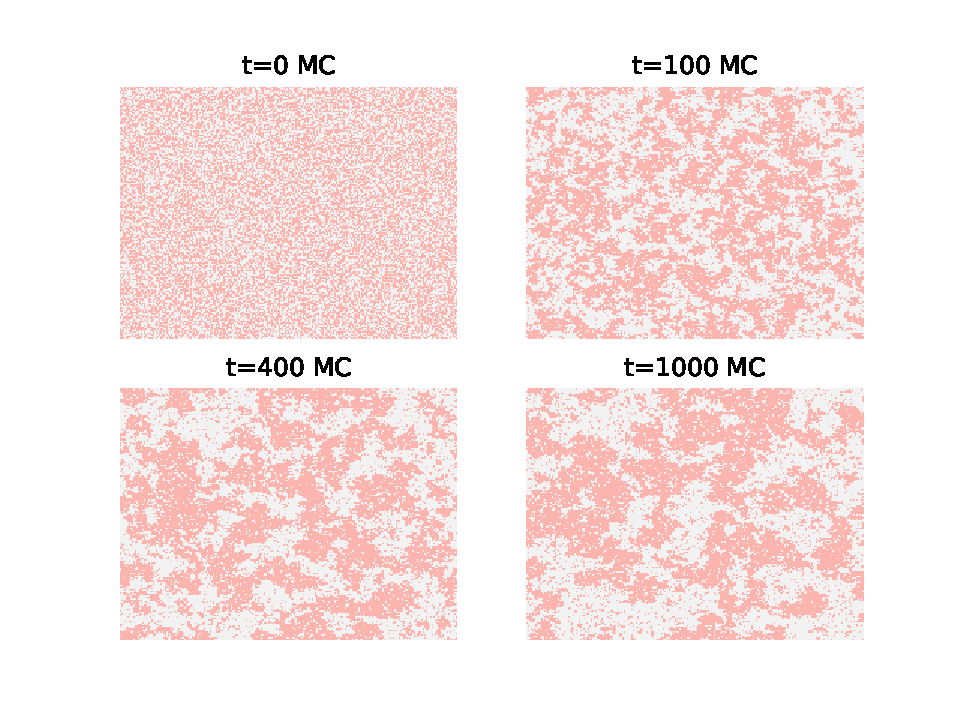
\includegraphics[width=0.9\linewidth]{intro/clusterization.pdf}
    \caption{Phénomène d'aggrégation à partir d'une trempe (\textit{quench}) dans un modèle d'Ising de $T=\infty$ à $T=T_C$ pour différents temps en étapes de Monte Carlo, pour un système $600 \times 600$ avec une dynamique non-conservée de Glauber.}
    \label{clusterization}
\end{figure}

%%%%%%%%%%%%%%%%%%%%%%%%%%%%%%%%%
\section{Équations dynamique d'un champ}
%%%%%%%%%%%%%%%%%%%%%%%%%%%%%%%%%

    \subsection{Champ avec un nombre de degrés de liberté fini}
Considérons un système dans l'ensemble canonique d'Hamiltonien  $H(\mq)$ où les $\mq_i$ ($i \in [0,N]$) représentent un nombre fini de degrés de liberté. La fonction de partition est donnée par 
\begin{align}
    Z = \int d\mq e^{-\beta H(\mq)}
\end{align}
avec la probabilité que le système se retrouve dans l'état $\mq$ égale à
\begin{align}
    P_{eq}(\mq) = \frac{e^{-\beta H(\mq)}}{Z}
    \label{eqdis}
\end{align}
À cause du trop grand nombre de degrés de libertés, la fonction de partition est rarement calculable analytiquement. Dans la limite $\beta \to \infty$ - c'est-à-dire la limite où la configuration du système minimisant le plus l'énergie est la plus probable - l'intégrale peut s'approcher par la méthode de Laplace pour l'évaluation des intégrales 
\begin{align}
    Z_{MF}= e^{-\beta H(\mq^*)}
\end{align}
Le champ $\mq^*$ est le champ qui minimise $H$ dont les degrés de liberté sont déterminés par
\begin{align}
    \frac{\partial H}{\partial q_i}|_{\mq={\bf q^*}}=0
\end{align}
Ce champ $\mq^*$ est le \textbf{champ moyen}, puisqu'il est le champ le plus probable. Dans cette approximation de champ moyen, toute observable est donnée par
\begin{align}
    < f(\mq) > = f(\mq^*)
\end{align}

On considère maintenant l'évolution temporelle du champ $\mq$ telle que son équation de Langevin donne la distribution à l'équilibre de Gibbs-Boltzmann : 
\begin{align}
    \frac{d q_i}{dt} = -L_{ij}\frac{\partial H(\mq)}{ \partial q_j} + \eta_i(t)
    \label{dynamique-langevin}
\end{align}
où $L_{ij}$ est un opérateur matriciel à définir et $\eta_i(t)$ un bruit blanc gaussien de fonction de corrélation
\begin{align}
   <  \eta_i(t)\eta_j(t') > =   \delta(t-t') \Gamma_{ij}
\end{align}
Le bruit blanc gaussien représente l'effef des fluctuations thermiques sur le système. On considère ici que le temps de corrélation de ces fluctuations est bien plus court que le temps charactéristique de l'évolution temporelle des degrés de liberté $q_i$, ce qui est de plus en plus vrai lorsque l'on se rapproche du point critique, à cause du ralentissement critique. Par symmétrie des fonctions de corrélation et de l'équation précédente nous pouvons en déduire que la matrice $\Gamma_{ij}$ doit être symmétrique et ne contenir que des valeurs propres positives.
À $T=0$, le système a tendance à minimiser son énergie, c'est-à-dire que
\begin{align}
    \frac{\partial H(\mq)}{ \partial q_j} = 0
\end{align}
Dans cette limite, l'équation \ref{dynamique-langevin} devient $\frac{d q_i}{dt}=0$, impliquant que le terme $\frac{\partial H(\mq)}{ \partial q_j}$ est le seul responsable de l'évolution du système.
Tant que la matrice $L_{ij}$ est inversible, la dynamique à $T=0$ fera tendre le système vers un minimum local de $H$, et vers son minimum global en absence de configurations métastables.
L'équation de Fokker-Planck de la densité de probabilité de la fonction des degrés de liberté $p(\mq,t)$ est 
\begin{align}
    \frac{\partial p(\mq,t)}{\partial t} = \frac{\partial}{\partial q_i} \left[\frac{1}{2}\Gamma_{ij}                 \frac{\partial p(\mq,t)}{\partial q_i} + p(\mq,t) L_{ij}\frac{\partial H(\mq)}{ \partial q_j}\right]
\end{align}
ou de manière plus concise
\begin{align}
    \frac{\partial p(\mq,t)}{\partial t} +\frac{\partial}{\partial q_i}J_i(\mq,t)=0
    \label{courant}
\end{align}
où  ${\bf J}(\mq,t)$ est le courant de probabilité. Le système respecte l'équilibre de Gibbs-Boltzmann si et seulement si $p(\mq,t)=P_{eq}(\mq)$ (donné par l'équation \ref{eqdis}) et que le courant soit nul, c'est-à-dire
\begin{align}
    \left[-\frac{\beta}{2}\Gamma_{ij} + L_{ij}\right]\frac{\partial H(\mq)}{ \partial q_j} = 0
\end{align}
Puisque cette relation est vraie quelque soit l'Hamiltonien considéré, on trouve  
\begin{align}
    \Gamma_{ij}= 2 k_B T L_{ij}
\end{align}
avec $k_B$ la constante de Boltzmann.

    \subsection{Théorie statistique des champs}

On considère maintenant un système d'Hamiltonien $H[\phi]$  dépendant d'un champ continu $\phi(\mx)$. Comme précédement, la fonction de partition est donnée par 
\begin{align}
    Z = \int d[\phi] e^{-\beta H[\phi]}
\end{align}
L'intégrale fonctionnelle sur tous les champs $\phi$ peut être prise dans la limite où $\phi$ est définie sur un réseau fini et où l'espacement entre chaque point tend vers $0$.
L'approximation du champ moyen devient maintenant
\begin{align}
Z _{MF}=  e^{-\beta H[\phi_{MF}]}
\end{align} 
où $\phi_{MF}$ est la solution de champ moyen qui minimise $H$, c'est-à-dire 
\begin{align}
    \frac{\delta H}{\delta\phi({\bf x})} = 0
\end{align}

Considérons maintenant l'Hamiltonien décrivant les modèles de type Ising
\begin{align}
    H[\phi] = \int d \mx  \frac{\kappa}{2}[\nabla \phi]^2 + V(\phi)
    \label{hamil-mean-field}
\end{align}
où le premier terme correspond à l'énergie d'interaction cherchant à diminuer les variations au sein du système, et le second terme est un potentiel symmétrique possédant deux minima globaux à basse température à $\pm \phi_C$ responsable de la séparation des phases, et possédant un minimum global à $\phi = 0$ à haute température. 

Par analogie avec le système avec un nombre fini de degré de libertés, on peut écrire l'équation de Langevin 
\begin{align}
    \frac{\partial \phi(\mx)}{\partial t}= -L \frac{\delta H}{\delta \phi(\mx)} + \eta(\mx,t).
\end{align}
avec la fonction de corrélation du bruit blanc gaussien
\begin{align}
    < \eta(\mx,t)\eta(\mx',t)> =\delta(t-t')\Gamma(\mx,\mx')
\end{align}
où  $L$ est un opérateur défini par son action sur la fonction $f$ comme
\begin{align}
    L f(\mx) = \int d\mx' L(\mx,\mx')f(\mx')
\end{align}
et de manière identique pour $\Gamma$.
De la même manière que précédement, on trouve que 
\begin{align} 
    \Gamma(\mx,\mx') =2 k_B T L(\mx,\mx')
\end{align}

Il est possible de choisir l'opérateur $L$ que l'on désire, puisque la distribution de Gibbs-Boltzmann à l'équilibre ne repose que sur la relation entre $L$ et $\Gamma$. 
Halperin et Hohenberg \cite{hohenberg_theory_1977} ont classifié les formes d'opérateurs les plus importants correspondant à des systèmes physiques.

La forme la plus simple est le \textbf{modèle A} donnée par $L(\mx,\mx')=\alpha\delta(\mx-\mx')$ 
\begin{align}
    \frac{\partial \phi(\mx)}{\partial t}= -\alpha \frac{\delta H}{\delta \phi(\mx)} + \eta(\mx,t)
    \label{MA}
\end{align}
de bruit blanc
\begin{align}
    < \eta(\mx,t)\eta(\mx',t)> =2T \alpha \delta(t-t')\delta(\mx-\mx').
\end{align}
On peut voir que la valeur moyenne $\overline \phi(t) = \frac{1}{V}\int d\mx \phi(\mx,t)$ n'est pas conservée. Le modèle A correspond alors à un système dans l'ensemble grand-canonique. Ici, le terme $\alpha$ est un coefficient cinétique décrivant le temps de relaxation du système. 
Le second modèle respectant les symmétries spatiales est le \textbf{modèle B}, et est donné par $L(\mx-\mx')= -D\nabla^2 \delta(\mx-{\bf x'})$ où le signe moins est nécessaire pour garantir la positivité de l'opérateur. On obtient l'équation d'évolution
\begin{align}
    \frac{\partial \phi(\mx)}{\partial t}= D\nabla^2 \frac{\delta H}{\delta \phi(\mx)} + \eta(\mx,t)
    \label{MB}
\end{align}
de bruit blanc
\begin{align}
    <\eta(\mx,t)\eta(\mx',t)> =-2TD   \delta(t-t')\nabla^2\delta(\mx-\mx')
\end{align}
En introduisant un bruit blanc vectoriel de composantes $\eta_i(\mx,t)$ tel que 
\begin{align}
    < \eta_i(\mx,t) \eta_i(\mx',t')> =\delta_{ij} \delta(\mx-\mx')\delta(t-t),
\end{align}
où $\delta_{ij}=1$ for $i=j$ et $0$ sinon, on peut maintenant écrire que 
\begin{align}
    \eta(\mx,t)= \nabla\cdot {\boldsymbol \eta}(\mx,t)
\end{align}
L'équation \ref{MB} devient 
\begin{align}
    \frac{\partial \phi(\mx)}{\partial t}= \nabla\cdot[ D\nabla \frac{\delta H}{\delta \phi(\mx)} + {\boldsymbol\eta}(\mx,t)]
\end{align}
Écrite sous cette forme, il est facile de voir que la valeur moyenne du paramètre d'ordre $\phi$ est conservé dans le temps. Le modèle B correspond à un système dans l'ensemble canonique, utile pour décrire les phénomènes de diffusion et d'accrétion.

À défaut de fluctuations thermiques, les équations \ref{MA} et \ref{MB} s'appellent respectivement les équations Ginzburg-Landau et de Cahn-Hillard \cite{cahn_free_nodate,langer_new_1975,kawasaki_growth_1978} et donnent l'évolution temporelle du champ moyen. 

    \subsection{Modèle $\phi^4$}
    
Le modèle standard, appelé $\phi^4$ est donné par le potentiel en double-puits de Landau-Ginzburg \cite[§ 45]{l_landau_physique_1990} 
\begin{align}
    V(\phi) = \frac{1}{2} m^2 \phi^2 + \frac{\lambda}{4!} \phi^4
    \label{phi4}
\end{align} 
où $m^2 = T-T_C$. À basse température, ce potentiel symmétrique possédant deux minima globaux à $\phi_C = \pm \sqrt{- \frac{6 m^2}{\lambda} } \pm$ décrit la séparation de phase.


Dans les expériences en laboratoire, les systèmes sont souvent couplés à des champs magnétiques ou chimiques $h(x)$ d'Hamiltonien
\begin{align}
    H_1 &= - \int d^dx h(\mx)\phi(\mx)
    \label{champ-externe}
\end{align}
qui induit un changement de stabilité entre les phases (voir Fig \ref{double-puits-temperature}). La nouvelle fonction de partition est
\begin{align}
    \mZ[h] = \int d [\phi] e^{ - \beta (\int d^d x \left( \frac{\kappa}{2} (\nabla \phi(\mx))^2 + V(\phi(\mx)) \right) + \beta \int d^d x h(\mx) \phi(\mx)}
\end{align}

\begin{figure}
    \centering
    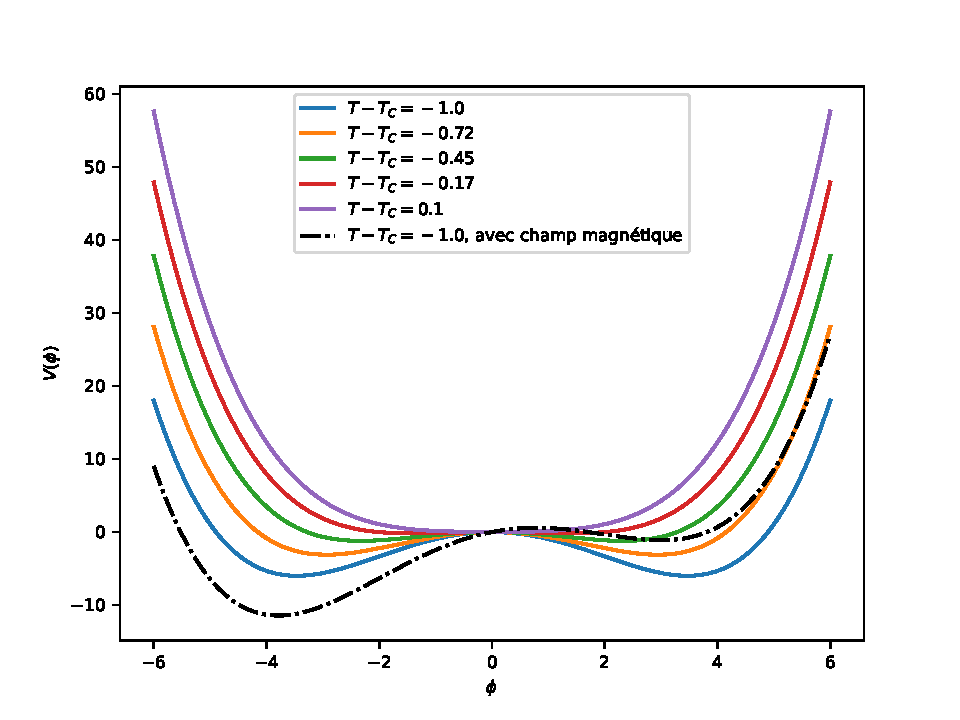
\includegraphics[width=0.6\linewidth]{intro/double-puit-en-fonction-temp.pdf}
    \caption{Potentiel en double-puits pour $\lambda=1$ en fonction de la différence entre la température et la température critique. Dans la phase ordonnée, les mimina stables sont à $\phi_C =\pm \sqrt{- \frac{3! m^2}{\lambda} } $ et à $\phi_C = 0$ pour la phase désordonnée. En noir, l'ajout d'un champ magnétique uniforme $h(\mx) = 1$ rend la phase positive métastable. {\color{red} $m^2 = T-T_C$, ref à l'équation}}
    \label{double-puits-temperature}
\end{figure}

La valeur moyenne de $\phi$ est alors
\begin{align}
    <\phi> =  \frac{1}{\mZ[h]} \int d [\phi] \phi(\mx)e^{ - \beta (\int d^d x \left( \frac{\kappa}{2} (\nabla \phi(\mx))^2 + V(\phi(\mx)) \right) + \beta \int d^d x h(\mx) \phi(\mx)}
\end{align}
Plaçons-nous maintenant dans la phase désordonnée, où $m^2 \ge 0$ et $\lambda \simeq 0$, ce qui nous permet d'avoir une approximation gaussienne. Si on réécrit l'Hamiltonien sous forme d'opérateurs, on obtient 
\begin{align}
    H[\phi] = \frac{1}{2} \int d^d x d^d y \; \phi(\mx) \mL(\mx,\my) \phi(\my) - \int d^d x h(\mx) \phi(\mx)
\end{align}
où l'on a introduit l'opérateur $\mL(\mx,\my) = (m^2 - \kappa \nabla^2) \delta(\mx-\my)$.
La fonction de partition prend maintenant la forme gaussienne
\begin{align}
    \mZ[h] \propto e^{- \frac{\beta}{2} \int d^d x d^d y h(\mx) \mL^{-1}(\mx,\my) h(\my)}
\end{align}
où $\mL^{-1}$ est déterminé par 
\begin{align}
    (m^2 - \kappa \nabla_\my^2) \mL^{-1}(\mx,\my) = \delta(\mx-\my)
\end{align}
Par identification avec la fonction de Green $\Gamma(\mx)$ de l'opérateur $m^2 - \kappa \nabla^2$, on obtient que l'énergie libre du modèle gaussien est au final donné par 
\begin{align}
    F[h] = F_0 - \frac{1}{2} \int d^d x d^dy \;  h(\mx) \Gamma(\mx-\my) h(\my)
\end{align}

La transformée de Fourrier de l'équation de la fonction de Green $(m^2-\kappa \nabla^2) \Gamma(\mx) = \delta(\mx)$ donne
\begin{align}
    \tilde{\Gamma}(\mq) = \frac{1}{\kappa} \frac{1}{\xi^{-2} +  q^2}
\end{align}
puis
\begin{align}
    \Gamma(\mx) = \frac{1}{\kappa} \int \frac{d^dq}{(2\pi)^d} \frac{e^{i \mq \cdot \mx}}{\xi^{-2} +  q^2}
    \label{fonction-correl}
\end{align}
où l'on a introduit la longueur de corrélation du système $\xi = \sqrt{\frac{\kappa}{m^2}}$.
Par ailleurs, par différentiation fonctionnelle directe de la fonction de partition, on voit que
\begin{align}
    <\phi(\mx)> = \frac{1}{\mZ[h]} \frac{1}{\beta} \frac{\delta \mZ[H]}{\delta h(\mx)} = \frac{\delta (k_B T \ln \mZ[h])}{\delta h(\mx)} = - \frac{\delta F}{\delta h(\mx)} = \int d^d \my \Gamma(\mx-\my) h(\my)
\end{align} 
avec l'énergie libre du système  $F[h] = -k_B T \ln(\mZ[h])$. Ce résultat n'est valable que pour $h \neq 0$ ou $h \to 0$. En absence de champ extérieur, la magnétisation est nulle.
De la même manière, on peut démontrer que la fonction de corrélation est égale à 
\begin{align}
    C(\mx,{\bf y}) =  <\phi(x)\phi(y)> = \frac{1}{\beta} \frac{\delta <\phi(\mx)>}{\delta h({\bf y})} = \frac{1}{\beta} \Gamma(\mx-\my)
\end{align}
et le facteur de structure
\begin{align}
    S(k) = < \tilde{\phi}(k)\tilde{\phi}(q)> = \frac{(2\pi)^d}{\beta} \delta(k-q)  \tilde{\Gamma}(\mq)
\end{align}
{\color{red} vecteurs k et q}
Dans la phase désordonnée, où $m^2 \less 0$ et $\lambda \neq 0$, l'approximation gaussienne du modèle $\phi^4$ donne le même résultat que \ref{fonction-correl} avec le facteur $m^2$ renormalisé par l'équation auto-consistante \cite[\P 4.3]{bellac_equilibrium_2004}
\begin{align}
    m^2_0 = m^2 + \frac{1}{2} \lambda \int_\mq \frac{1}{m^2_0+\mq^2}
\end{align}
    \subsection{Tension superficielle}

La solution de champ moyen minimise l'Hamiltonien \ref{hamil-mean-field},  nous donne
\begin{align}
    \frac{\delta H}{\delta \phi(\mx)} = -\kappa \nabla^2 \phi(\mx) + V'(\phi)
    \label{interface}
\end{align}
Puisque le potentiel $V(\phi)$ est supposé symmétrique et possédant deux minima globaux en $\pm \phi_C$, en l'absence de contrainte, le système tend vers la solution homogène $\phi(\mx) = \pm \phi_C$ correspondant à l'énergie libre $F=H[\phi_C]=0$. Néanmoins, dans le cas où le paramètre d'ordre est conservé
\begin{align}
    \int d \mx \phi(\mx)=0
\end{align}
la solution $\phi(\mx)=\pm \phi_c$ est impossible. Dans ce cas, le système va se séparer en plusieurs phases homogènes $\phi(\mx)= \pm \phi_c$. 
Plaçons-nous au voisinnage de l'interface entre deux phases, c'est-à-dire que le champ $\phi$ est invariant par translation en $x$ et $y$ et que la longueur de corrélation $\xi$ est bien plus grande que la taille de l'interface, c'est-à-dire que $\phi(\mx) = \phi_K(z)$ (où $K$ désigne un \textit{kink}) et $\lim_{z\to\-\infty}=-\phi_c$ and  $\lim_{z\to\infty}=-\phi_c$, ce qui nous donne d'après \ref{interface}
\begin{align}
    \kappa \phi_K''(z) =  V'(\phi_K)
    \label{kink}
\end{align}
En multipliant de chaque côté par $\phi'_K(z)$ et en utilisant les conditions aux limites, on trouve que 
\begin{align}
    H[\phi_K]=  A\int dz\ \kappa \phi_K'^2(z)
\end{align}
où $A$ est l'aire de la surface du système dans le plan perpendiculaire à la direction $z$. On peut identifier l'intégrale à une énergie libre par unité de surface, c'est à dire la tension superficielle de l'interface $\sigma$ définie par l'équation d'Allen-Cahn
\begin{align}
    \sigma=  \int dz\ \kappa \phi_K'^2(z)
    \label{tension-superficielle}
\end{align}
Il s'ensuit que l'excès d'énergie est localisé au niveau de l'interface, et que la force principale de la croissance des domaines est la courbure du profil de l'interface, puisque l'énergie du système ne peut diminuer que par une réduction de l'aire totale de l'interface. 

Dans le cas du modèle $\phi^4$ définie à l'équation \ref{phi4}, l'équation \ref{kink} devient
\begin{align}
    \kappa \phi_K''(z) = \phi_K(z) \left( m^2 + \frac{\lambda}{3!} \phi_K(z) ^2 \right)
       \label{eq-interface-glauber}
\end{align}
dont la solution est
\begin{align}
    \phi_K(z) = \phi_C \tanh \left( \frac{z}{\sqrt{\frac{-m^2}{2 \kappa}}} \right)
       \label{profil-interface-glauber}    
\end{align}


%%%%%%%%%%%%%%%%%%%%%%%%%%%%%%%%%
    \section{Taille finie et effet Casimir critique}
    \label{sec-casimir}    
%%%%%%%%%%%%%%%%%%%%%%%%%%%%%%%%%
    
Supposons un système 2D de taille $L \times L' $ où $L \less L'$. L'énergie libre $F(\beta,L,L') = - \frac{1}{\beta} \ln ( Z(\beta,L,L'))$ est une grandeur extensive lorsque la longueur de corrélation est plus petite que la taille du système $L$. 
Cette énergie libre peut se décomposer entre l'énergie de chaque phase par unité de volume $\omega_{bulk}$, et l'énergie de tension superficielle à l'interface par unité de surface $\omega_{surf}$ \cite{cardozo_finite_2015,lopes_cardozo_critical_2014}. À noter qu'à haute température dans un système complètement homogène, ce dernier terme disparaît.

Cependant, lorsque $\xi \simeq L$, la contrainte exercée sur les fluctuations thermiques par les conditions aux bords implique une modification de l'énergie libre, créant une force sur les parois. Cet effet, premièrement prédit par Hendrik Casimir\cite{h_b_g_casimir_attraction_1948}, fut étendu aux systèmes critiques, où la divergence de la longueur de corrélation rend les expériences bien plus faciles\cite{nguyen_controlling_2013}.
{\color{red} réf originale de gennes fischer, ref 15 cardozo, review gambassi}
{\color{red} résumé notes David Casimir}

En présence d'un champ magnétique $h$ uniforme favorisant une phase par rapport à l'autre, l'énergie libre par unité d'aire d'un tel système se décompose \cite{lopes_cardozo_critical_2014,cardozo_finite_2015} en 
\begin{align}
    \frac{\Omega(\beta,L,L',h)}{L'} = L \omega_{bulk}(\beta,h) + \omega_{surf}(\beta,h) + L \omega_{ex}(\beta,L,h)
    \label{decomposition-energie}
\end{align}
où $\omega_{ex}(L,h)$ est le surplus d'énergie libre due au confinement des fluctuations, qui devient nul dans la limite $L\to \infty$.

La force de confinement par unité d'aire est définie par 
\begin{align}
    F_\perp(\beta,L,h) = - \frac{1}{L' }\frac{\partial \Omega(\beta,L,h)}{\partial L} \bigg|_{\beta,L'} = - k_B T \omega_{bulk}(\beta,h) - k_B T \frac{\partial(L \omega_{ex}(\beta,L,h))}{\partial L}\bigg|_{\beta,L'}
\end{align}
où le premier terme est la pression exercée par le système, tandis que le second terme est la force de Casimir par unité d'aire \cite{vasilyev_critical_2013} en $d$ dimensions 
\begin{align}
    f_c(\beta,L,h) = - k_B T \frac{\partial(L \omega_{ex}(\beta,L,h))}{\partial L}\bigg|_{\beta,L'} = k_B T L^{-d} \Theta(u_t,u_h)
    \label{casimir-scaling}
\end{align}
où $u_T = \frac{T-T_C}{T_C} L^\frac{1}{\nu}$ et $u_h = \frac{h}{k_B T_C} L^\frac{\beta+\gamma}{\nu}$ et où les exposants $\beta$, $\gamma$ et $\nu$ sont des exposants universels reliés aux amplitudes universelles des longueurs de corrélation du système \cite{pelissetto_critical_2002,vasilyev_critical_2013} et $\Theta(u_t,u_h)$ est une fonction universelle propre à chaque modèle. Cette fonction universelle dépend des conditions aux bords du système \cite{dantchev_casimir_2017,dantchev_exact_2016} ainsi que de l'ensemble thermodynamique dans lequel on se place \cite{gross_critical_2016,rohwer_transient_2017}.

Afin d'extraire la force de Casimir, il suffit alors de soustraire deux quantités extensives, c'est-à-dire en utilisant deux largeurs différentes $L_1$ et $L_2$
\begin{align}
    f_c(\beta,L_1,h) - f_c(\beta,L_2,h) =  \frac{1}{L' }\frac{\partial \Omega(\beta,L_2,h)}{\partial L} \bigg|_{\beta,L'} -  \frac{1}{L' }\frac{\partial \Omega(\beta,L_1,h)}{\partial L} \bigg|_{\beta,L'}
\end{align}
Puisque le surplus d'énergie dû au confinement est nul lorsque $L_2\to \infty$, on obtient que la force de Casimir est
\begin{align}
    f_c(\beta,L_1,h) \simeq \frac{1}{L' }\frac{\partial \Omega(\beta,L_2,h)}{\partial L} \bigg|_{\beta,L'} -  \frac{1}{L' }\frac{\partial \Omega(\beta,L_1,h)}{\partial L} \bigg|_{\beta,L'}
    \label{casimir-diff-omega}   
\end{align}
où en utilisant \ref{casimir-scaling}, l'approximation est valable dans le cas où $ \left( \frac{L_2}{L_1}\right)^{-d} \ll 1 $.  Cette force étant une force émergente d'origine entropique, la somme des forces exercées individuellement par chaque particule du système n'est pas égale à la force totale appliquée sur le système\cite{paladugu_nonadditivity_2016}.

La détection expérimentale de ce phénomène se fait traditionnellement dans des fluides binaires par \textit{Total Internal Reflection Microscopy} (TIRM) \cite{fukuto_critical_2005,hertlein_direct_2008,gambassi_critical_2009,edison_critical_2015-1}. La méthode consiste à mesurer le potentiel d'une sphère flottant sur un fluide binaire critique reposant sur une plaque. Cette sphère et cette plaque sont traitées chimiquement afin de favoriser l'une des deux phases à leu voisinage. Ainsi il est possible de créer des conditions aux bords $(++)$, $(+-)$ ou $(--)$ qui modifient la forme de la fonction universelle \ref{casimir-scaling}. À l'inverse, il est possible de mesurer la force de Casimir \cite{nguyen_controlling_2013} afin d'étudier les transitions de phases colloïdales.

Le modèle d'Ising appartient à une classe de modèles où il est facilitant l'obtention de résultat analytique \cite{hobrecht_critical_2017} comparables aux simulations numériques \cite{vasilyev_monte_2007,vasilyev_universal_2009,cardozo_finite_2015}.

Jusqu'à présent nous avons parlé de systèmes à l'équilibre, mais l'effet des fluctuations est également présent en dehors de l'équilibre. L'étude des interfaces nous mène à proposer des modèles de cisaillement qui influencent les propriétés statistiques des systèmes, et ainsi modifier la force de Casimir \cite{dean_out--equilibrium_2010}.

    \section{Modèles d'interface}

Dans la réalité, la phase désordonnée est extrêmement inhomogène, avec des bulles ou des digitations qui empêchent une description dynamique aisée de l'interface. Si l'on désire étudier l'interface de ces bulles ou digitations, où localement l'interface est bien définie par une fonction d'une seule variable, l'approche du champ moyen suffit. On suppose dans ce cas qu'il n'y a ni digitation ni bulles d'évaporation. Dans cette approximation, l'interface est parfaitement définie en un point et non dans un profil comme dans l'équation \ref{profil-interface-glauber}. Tous les points du champ se trouvant en bas de l'interface prennent une unique valeur strictement différente de tous les points du champ au-dessus de l'interface. 

Sans perte de généralité, nous pouvons séparer les variables spatiales par $x$ pour toutes les coordonnées parallèles à l'interface et par $z$ la coordonnée transverse. Cela se traduit par
\begin{align}
    \phi(\mx,z) = f(z-h(\mx))
    \label{capillary-wave-theory}
\end{align}
où $f(a \greater 0) = \phi_1$ et $f(a \less 0) = \phi_2$. Notre système est maintenant complètement défini par l'interface $h(x)$ d'Hamiltonien
{\color{red} $\phi$ miminise champ moyen }
\begin{align}
    H = \int d^d x \frac{\sigma}{2} (\nabla h(\mx))^2 + V(h(\mx))
    \label{hamil-cwt}
\end{align}
{\color{red} expliquer développement pour surface dans formule de Mange}

où le premier terme est l'excès d'énergie par rapport à une interface plane, et le potentiel $V$ fait référence au champ externe \ref{champ-externe}. 
Une interface se caractérise par sa hauteur moyenne $<h(t)>$ de l'interface dans l'espace et par sa fonction de corrélation parallèle à l'interface décrivant les modes de fluctuation de l'interface
\begin{align}
    C_\parallel(r,t) = <h(\mx,t)h(\mx+r,t)>_x - <h(0,t)>^2 = \sum_i A_i(\frac{r}{\xi_i}) 
\end{align}
où les $A_i$ sont des fonctions à décroissance exponentielle. Le calcul de ces fonctions sera donnée dans la section \ref{sec_laser}. 
L'épaisseur de l'interface est donnée par $\omega(t) = \sqrt{C_\parallel(0,t)} = \sqrt{<h(t)^2> - <h(t)>^2}$. 

    \subsection{Paramètre d'ordre non conservé}

Supposons une surface à laquelle viennent s'agréger des particules provenant d'un réservoir afin de créer un dépot. L'interface est alors définie par la hauteur de l'aggrégat par rapport à la surface de dépôt.

En partant de \ref{MA} et en insérant \ref{capillary-wave-theory} avec le changement de variable $u= z-h$, on a \cite{bray_interface_2001}
\begin{align}
    \frac{\partial h}{\partial t} f'(u) &= D \nabla^2 h f'(u) - V'(f) + \eta(\mx,u+h(\mx,t),t)
\end{align}
avec $\eta(x,t)$ un bruit blanc gaussien. En multipliant les deux côtés par $f'(u)$ et en intégrant de $-\infty$ à $+\infty$, puisque le terme $ \int_{-\infty}^\infty V'(f) f'(u) du = 0$, on obtient l'équation d'Edwards-Wilkinson \cite{edwards_surface_1982} 
\begin{align}
     \frac{\partial h}{\partial t} = \nu + \nabla^2 h +  \tilde{\eta}(\mx,t)
    \label{edwards-wilkinson}
\end{align}
{\color{red} ne pas mettre $\nu$, on s'emballe ??? gné ? voir notes de David. Éliminer la section, rmeplacer avec la dérivation dans les notes}
où $\nu$ désigne le flux total, et $\tilde{\eta}(x,t)$  un bruit blanc de moyenne nulle défini par
\begin{align}
    \tilde{\eta}(\mx,t) = - \frac{1}{\sigma} \int du f'(u) \eta(\mx,u+h(\mx,t),t)
\end{align}
et de corrélation 
\begin{align}
    <\tilde{\eta}(\mx,t)\tilde{\eta}(\mx',t')> = \frac{2 D}{\sigma} T\delta(\mx-\mx')\delta(t-t')
\end{align}
avec $\sigma$ la tension superficielle définie en \ref{tension-superficielle}, et $D$ le bruit thermique.
Ici $D+ \sqrt{2 D T} \tilde{\eta}(x,t)$ est le flux de particules s'aggrégeant en fonction du temps et $D \nabla^2 h$ dépend de la forme de l'interface, favorisant ou non le dépôt de particules à certains endroits.
La hauteur moyenne de l'interface varie donc comme $<h(t)> = \nu t$. En se positionant dans le référentiel de l'interface via la transformation $h \rightarrow h + \nu t$, on obtient
\begin{align}
     \frac{\partial h}{\partial t} =    \nabla^2 h +  \tilde{\eta}(\mx,t)
    \label{edwards-wilkinson-conesrved}
\end{align}

    \subsection{Paramètre d'ordre conservé}

Si l'on se place dans le référentiel du centre de l'interface, le'équation d'Edwards-Wilkinson \ref{edwards-wilkinson-conesrved} conserve le paramètre d'ordre en moyenne. Néanmoins, la transformation $h \rightarrow h + Dt$ ne prend pas en compte les fluctuations thermiques qui viennent perturber l'interface, ce qui fait que $h(t) \neq cte$. L'astuce vient ici de \cite{kawasaki_diffusion_1966,kawasaki_correlation-function_1966}, où l'on reprend l'équation de Cahn-Hilliard-Cook \ref{MB} pour les interfaces
\begin{align}
    \frac{\partial h}{\partial t} =  \nabla^2 \frac{\delta H}{\delta h} +  \tilde{\eta}(x,t)
\end{align}
{\color{red}$ H =\int d \mx \frac{\sigma (\nabla h)^2}{2} +V(h(x) $}
{\color{red} version modèle de KPZ, pas le moême modèle. Enlever $\nabla^2 (\nabla h)^2$}
qui nous donne l'équation Villain-Lai-Das Sarma\cite{villain_continuum_1991,lai_kinetic_1991}
\begin{align}
    \frac{\partial h}{\partial t} = - \nabla^4 h + \lambda \nabla^2 (\nabla h) ^2 +  \tilde{\eta}(x,t)
\end{align}
qui a fait l'objet de nombreuses études\cite{kim_conserved_1994,assis_dynamic_2015,oliveira_maximal-_2008,singha_renormalization_2016}.
L'intérêt d'un tel système est qu'il est contraint à une dynamique locale qui permet d'obtenir un système hors-équilibre. 

    \subsection{Interface hors équilibre}

Les systèmes à l'équilibre ont la particularité que les états ont une probabilité en accord avec la distribution de Gibbs-Boltzmann \ref{eqdis}, c'est-à-dire que le courant \ref{courant} est nul. La manière la plus simple de mettre le système hors-équilibre est donc d'induire un courant dans le champ $\phi(\mx,t)$. L'évolution d'un système depuis une condition initiale vers ses configurations d'équilibre est le moyen le plus simple d'étudier les conditions hors équilibre. On retrouve également dans le régime stationnaire beaucoup de systèmes hors-équilibre. Expérimentalement, les colloïdes sédimentant dans un champ gravitationel induisent un écoulement hors-équilibre. Il est également possible d'induire un flux sur des particules chargées dans un champ électrique via la pression de radiation exercée par un laser ou par un cisaillement dans un liquide visqueux\cite{girot_conical_2019}. Cette dynamique étant locale, elle ne peut exister que si le paramètre d'ordre est conservé. L'équation générale d'un système d'interface avec un cisaillement est\cite{bray_interface_2001-1,bray_interface_2001}
\begin{align}
     \frac{\partial h}{\partial t} + v \nabla h =  \mathcal{L} h +  \eta(x,t)
     \label{eq-cisaillement}
\end{align}
{\color{red} $v \nabla h$ are vectors scalar product $\nabla (vh)$ vecteur advection du à un écoulement. Mettre la formule pour un cisaillement, article Bray. Dire que champ de vitesse est constant pour faire transfo galiliéenne, écrire qu'est-ce que c'est que le cisaillement. 
Champ de cisaillement c'est à revoir}
où l'opérateur $\mathcal{L}$ est associé au modèle A ou B, et le terme $v \nabla h$ est un terme de d'advection dû au flux produit par le cisaillement. 

Dans le cas où le champ de vitesse est constant, comme la sédimentation dans un champ gravitationel, on peut parler d'écoulement. L'équation \ref{eq-cisaillement} est alors invariante par la transformation galiléenne $x \rightarrow x+vt$. 

\begin{figure}
	\begin{minipage}[t]{0.5\linewidth}
		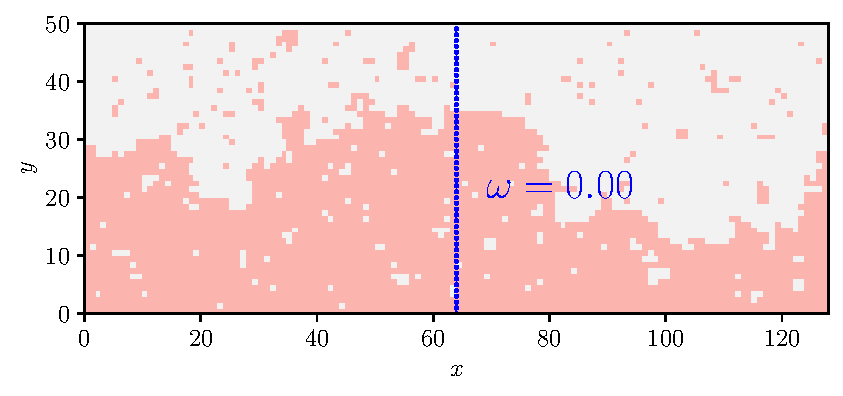
\includegraphics[width=\linewidth]{intro/cis-ising-f-000.pdf}
	\end{minipage}%
	\begin{minipage}[t]{0.5\linewidth}
		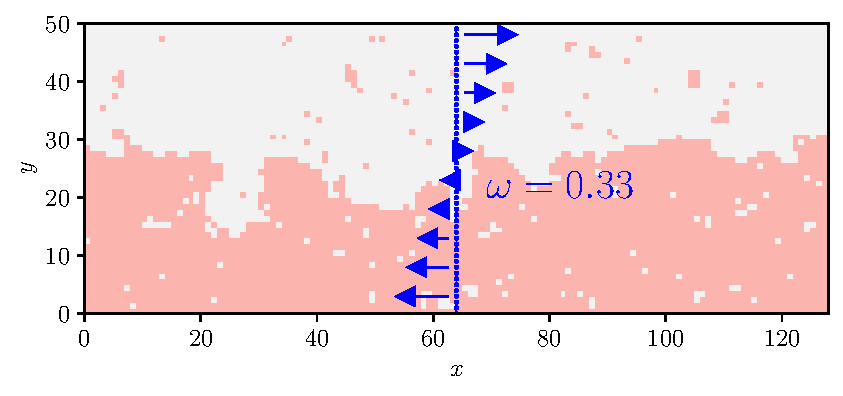
\includegraphics[width=\linewidth]{intro/cis-ising-f-033.pdf}
	\end{minipage}
	\centering
	\begin{minipage}[t]{0.5\linewidth}
		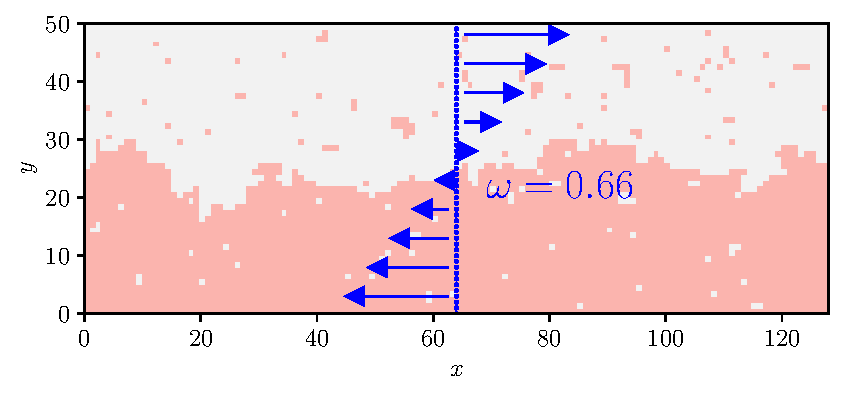
\includegraphics[width=\linewidth]{intro/cis-ising-f-066.pdf}
	\end{minipage}
	\caption{Photos d'un système d'Ising $128 \times 50$ en fonction d'un cisaillement
	${f(y) = \omega (\frac{2 y}{L} -1)}$.  {\color{red} expliquer qu'est-ce qu'un cisaillement, comment on implémente ça dans un modèle discret}}
    \label{snap-ising-shear}	
\end{figure}  

\begin{figure}
    \centering
    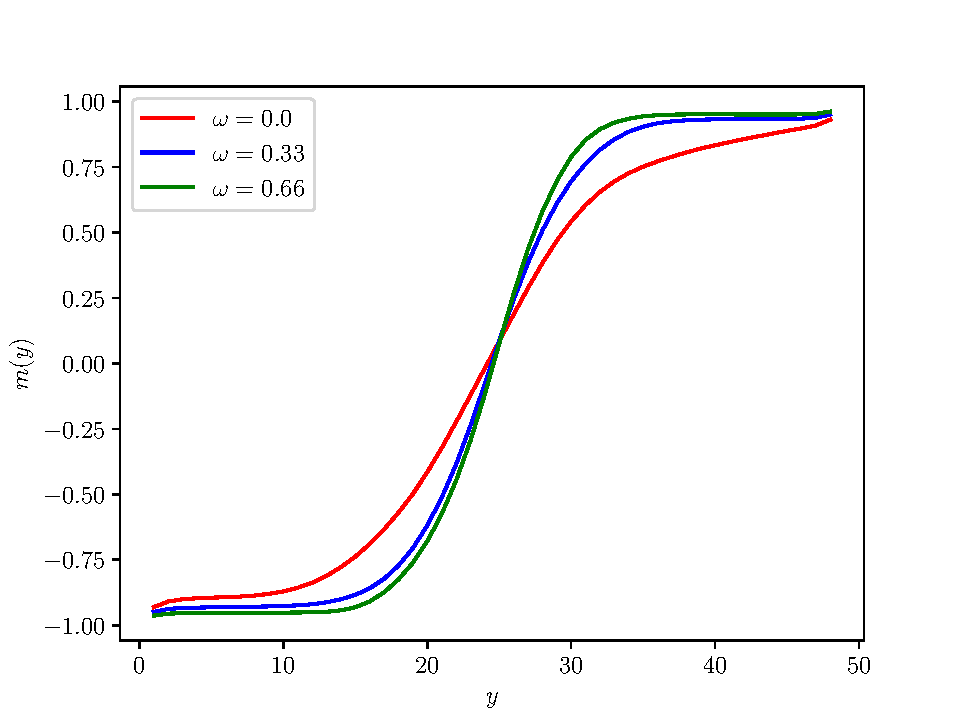
\includegraphics[width=0.6\linewidth]{intro/profil-mag-ising-shear.pdf}
    \caption{Profil de magnétisation d'un système d'Ising $128 \times 50$ en fonction du cisaillement de la figure \ref{snap-ising-shear}. Plus le cisaillement est élevé, plus l'interface est confinée.}
    \label{profil-mag-ising-shear}
\end{figure}

Néanmoins, de nombreuses expériences\cite{derks_suppression_2006} et simulations numériques pour le modèle d'Ising \cite{leung_field_1986,rikvold_microstructure_2002,gonnella_nonequilibrium_2009,smith_driven_2010,smith_interfaces_2008,sadhu_non-local_2014,cohen_interface_2016,cirillo_monte_2005} ainsi qu'avec des techniques de Dynamique Moléculaire \cite{berthier_nonequilibrium_2002} montrent que le cisaillement provoque un confinement de l'interface. Dans les expériences où les effets gravitationnels sont importants, le solvant d'une suspension de colloïdes ne bouge pas, contrairement aux particules en suspension. La brisure d'invariance galiléenne qui en résulte est expliqué en détail au chapitre \ref{chap-article-dean}. \footnote{Ce chapitre a été publié dans \cite{dean_effect_2020}.}
Pour les simulations de Monte Carlo, l'invariance est brisée par la dynamique même du système, puisque les mouvements sont fait séquentiellement et non simultanément.

\section{Conclusion}

Nous avons présenté les modèles standards des transitions de phase et avons étudié l'importance de l'ensemble thermodynamique de ces systèmes.
Dans l'ensemble grand-canonique où le paramètre d'odre n'est pas conservé, les équations dynamiques du modèle A \ref{MA} appliqués au champ $\phi(\mx,t)$ permettent de calculer la fonction de corrélation du système pour le modèle $\phi^4$. Le modèle $\phi^4$ permet de basculer naturellement vers un modèle d'interface $h(\mx,t)$ qui réduit la dimensionalité du champ et rend ainsi les calculs plus simples.
	Il existe par ailleurs de nombreuses sources contribuant à l'énergie totale du système : l'énergie du volume (\textit{bulk}) du système, l'énergie de l'interface définie par sa tension superficielle \ref{tension-superficielle}, et une énergie d'excès qui donne naissance à la force de Casimir \ref{casimir-scaling}. Cette force est dûe au confinement du système par des conditions aux bords contraignant les fluctuations du champ $\phi$ selon une direction. 


Dans l'esemble canonique où le paramètre d'ordre est conservé (ou modèle B \ref{MB}), toutes les considérations antérieures se s'appliquent. Il est possible d'appliquer un flux local qui sort le système de l'équilibre. La manière la plus naturelle de le faire est de cisailler l'interface, ce qui modifie également les propriétés statistiques du système. 

Nous nous intéressons maintenant aux modèles sur réseaux, qui présentent l'avantage de la simplicité numérique et analytique et permettent de modifier facilement l'ensemble thermodynamique ainsi que le cisaillement. 